\chapter{Graph neural networks and deep reinforcement learning}
\label{chap:math}

Deep learning and neural networks have achieved unprecedented success since their introduction and currently are state-of-the-art in numerous fields, such as object detection \cite{DBLP:journals/corr/RedmonDGF15, 10.1109/IVS.2019.8813777, 8627998}, machine translation \cite{DBLP:journals/corr/LuongPM15, 8003957, DBLP:journals/corr/abs-2002-07526}, and many others \cite{DONG2021100379, 10.1145/3505243, PICCIALLI2021111}. Many deep learning techniques involve learning from Euclidian data (e.g., images, text, and videos). At the same time, there is an increasing number of fields where data is represented as graphs. For example, the interaction of users on social media \cite{10.1145/3308558.3313488}, atoms and their bonds in protein molecules \cite{strokach2020fast}, and traffic forecasting \cite{JIANG2022117921}. Learning from graph data has created significant challenges. Graphs can be irregular, with varying numbers of nodes, and each node can have a different number of neighbors. As a result, some important operations (e.g., convolution) can not be applied the same way as in the case of images. With growing interest in deep learning from graph data, new methods motivated by Convolutional Neural Networks and Recurrent Neural networks have been developed. For example, an image can be thought of as a graph, where each node is a pixel, and edges connect nodes partaking in convolution, as illustrated in Figure 2.1 below \cite{9046288}.\\
\begin{center}
    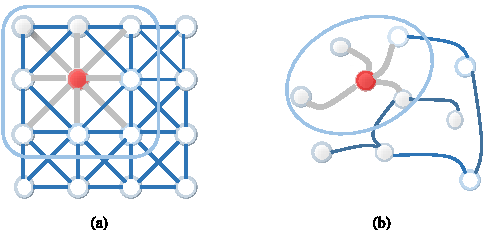
\includegraphics[width=0.6\linewidth]{images/image_vs_graph.pdf}\\
    Figure 2.1: 2-D Convolution versus graph convolution \cite{9046288}
\end{center}
\newpage
Similarly, for text processing and RNNs, text can be thought of as a graph, where each node is a word in a sentence, and every two consecutive words are connected via an oriented arc, as illustrated in Figure 2.2 below \cite{sanchez-lengeling2021a}.
\begin{center}
    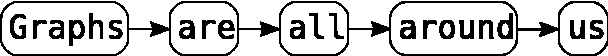
\includegraphics[width=0.7\linewidth]{images/graph_are_all_around_us.pdf}\\
    Figure 2.2: Text as a graph, reproduced from \cite{sanchez-lengeling2021a}
\end{center}

\section{Graph Neural Networks}

In the simplest case, when data is represented as a non-oriented graph $G = (O, E)$, each node $o \in O$ has a set of features $\vec{x}_o$. For example, the processing time of each operation node in the JSSP disjunctive graph. 
\par
A Graph Neural Network (GNN) takes this graph as an input and processes its features in two phases. The first phase, called \textit{message passing phase} \cite{pmlr-v70-gilmer17a}, runs for $K$ steps and uses a message function $M_{(k)}$ and a node update function $U_{(k)}$. In each step $k$, for each node $o$, a message $\vec{m}_o^{(k + 1)}$ is calculated, and the embedding of the node $\vec{h}_o^{(k)}$ is updated according to \cite{pmlr-v70-gilmer17a}
\begin{equation}\label{equation:2.1}
	\vec{m}_o^{(k + 1)} = \sum_{w \in \mathcal{N}(o)} M_{(k)} \left(\vec{h}_o^{(k)}, \vec{h}_w^{(k)}\right) \hspace{2em} \forall o \in O \, ,
\end{equation}
\begin{equation}\label{equation:2.2}
	\vec{h}_o^{(k+1)} = U_{(k)} \left(\vec{h}_o^{(k)}, \vec{m}_o^{(k+1)}\right) \hspace{2em }\forall o \in O \, , 
\end{equation}
where $\mathcal{N}(o)$ in the sum defines the neighbourhood of the node $o$ in graph $G$. The initial embedding of the node is $\vec{h}_o^{(0)} = \vec{x}_o$. Each step is often called a \textit{layer} of GNN.
\par
In the \textit{readout phase}, a readout function $R$ computes a vector $\vec{z}_o$ from obtained node embeddings \cite{pmlr-v70-gilmer17a}
\begin{equation}\label{equation:2.3}
	\vec{z}_o = R\left(\vec{h}_o^{(K)}\right) \hspace{2em} \forall o \in O \, .
\end{equation}
Message function $M_{(k)}$, node update function $U_{(k)}$, and readout function $R$ can all be parametrized differentiable functions. Each layer can have different parameters for these functions.
\par
Different forms of equations \ref{equation:2.1}, \ref{equation:2.2}, and \ref{equation:2.3} lead to different types of GNNs performing different tasks, for example, Graph Convolutional Neural Networks, Graph Recurrent Neural Networks, and Graph Attention Networks \cite{sanchez-lengeling2021a, 10.1145/3495161, DBLP:journals/corr/abs-1810-00826}. This thesis will focus primarily on relevant GNN architectures used in available job scheduling models described in the next chapter, specifically Graph Isomorphism Network and Graph Attention Network.

\subsection{Graph Isomorphism Network} \label{graph Isomorphism network}
Graph Isomorphism Network (GIN) is a GNN variant, where in the message passing phase, the update function $U_{(k)}$ is represented by a multi-layer perceptron $\text{MLP}^{(k)}$, and the equation \ref{equation:2.2} has the following form \cite{DBLP:journals/corr/abs-1810-00826}
\begin{equation} \label{equation:2.4}
	\vec{h}_o^{(k+1)} = \text{MLP}^{(k)} \left ( \left ( 1 + \epsilon^{(k)} \right ) \vec{h}_o^{(k)} + \sum_{w\in \mathcal{N}(o)} \vec{h}_w^{(k)} \right ) \, ,
\end{equation}
where $\epsilon^{(k)}$ can be learned or a fixed scalar \cite{DBLP:journals/corr/abs-1810-00826}. In the readout phase, the readout function $R$ depends on the model's given task, e.g., node classification, link prediction, and graph classification \cite{DBLP:journals/corr/abs-1810-00826}. Readout functions will be specified for each model separately in the next chapter.
\par
A straightforward strategy to extend GIN to directed graphs $G = (O, A)$ is to define the neighborhood of node $o \in O$ as $\mathcal{N}(o) = \{ w | \ (w, o) \in A\}$, i.e., all incoming neighbors of $o$ \cite{zhang2020learning}.\\
\\
For GIN on heterogeneous graphs, the equation \ref{equation:2.4} is applied separately for each type of neighbor node and then combined \cite{10226873, pytorch_hetero_conv}. Let $a$ denote a type of node $o$, $b$ denote a type of node $w$, and $r$ be an edge type connecting nodes of types $a$ and $b$. Then, let neighborhood $\mathcal{N}_{r}(o)$ be a set of nodes $b$ connected to $o$ by an edge of type $r$. Then, for each edge type $r$, updated embedding $\vec{h}_{o, r}^{(k+1)}$ of node $o$ is calculated by equation \ref{equation:2.4} separately (with separate multi-layer perceptrons) as follows \cite{pytorch_hetero_conv}
\begin{equation} \label{equation:2.5}
	\vec{h}_{o, r}^{(k+1)} = \text{MLP}^{(k)}_{r} \left ( \left ( 1 + \epsilon_{r}^{(k)} \right ) \vec{h}_{o}^{(k)} + \sum_{w\in \mathcal{N}_{r}(o)} h_{w}^{(k)} \right ) \, ,
\end{equation}
where $\text{MLP}^{(t)}_{r}$ is a multilayer perceptron for edge type $r$ \cite{pytorch_hetero_conv}. New embeddings for the node for each edge type $\vec{h}_{o, r}^{(k+1)}$ are then combined via some aggregation function \cite{pytorch_hetero_conv}, for example, a sum.

\subsection{Graph Attention Network}
Graph Attention Network (GAT) is a graph neural network architecture leveraging an attention mechanism \cite{veličković2018graph}. In each step (layer) $k$, nodes assign different importance weights to different nodes in their neighborhood by attending over their features. In job scheduling, higher importance weights may be assigned to operations expected to start sooner \cite{9826438}.
\par
In the first step, \textit{attention coefficients} $e_{ij}$ are computed as follows \cite{9826438, veličković2018graph}
\begin{equation} \label{equation:2.6}
	e_{ow} = a\left ( \boldsymbol{W} \vec{h}_o^{(k)}, \boldsymbol{W} \vec{h}_w^{(k)}  \right ) \, ,
\end{equation}  
where $a$ is a shared attention mechanism, and $\boldsymbol{W}$ is a shared learnable linear transformation. The attention mechanism $a$ is usually a single-layer feedforward neural network parametrized by a learnable vector $\vec{b}$ with LeakyReLU activation \cite{9826438, veličković2018graph, DBLP:journals/corr/abs-2105-14491}
\begin{equation} \label{equation:2.7}
	e_{ow} = \text{LeakyReLU}\left ( \vec{b} \cdot \left [ \boldsymbol{W}\vec{h}_o^{(k)} || \boldsymbol{W}\vec{h}_w^{(k)} \right ] \right ) \, ,
\end{equation}
where $\bullet||\bullet$ represents concatenation, and $\text{LeakyRELU} = \text{max}(cx,x)$ with $c \in [0,1]$ \cite{leaky_relu}.
\par
Then, the attention coefficients are normalized using the Softmax function only across the neighborhood and the node itself \cite{9826438, veličković2018graph}
\begin{equation}
	\alpha_{ow} = \frac{\exp(e_{ow})}{\sum_{q \in \mathcal{N}(o)} \exp(e_{oq})} \hspace{2em} \forall w \in \mathcal{N}(o) \cup {o} \, .
\end{equation}
As the last step, GAT computes a new node embedding as follows \cite{9826438, veličković2018graph}
\begin{equation} \label{equation:2.9}
	\vec{h}_o^{(k+1)} = \sigma \left ( \sum_{w \in \mathcal{N}(o) \cup {o}} \alpha_{ow} \boldsymbol{W} \vec{h}_w^{(k)} \right ) \, ,
\end{equation}
where $\sigma$ is an activation function. 
\par
It is also possible to use \textit{multi-head attention} to stabilize the learning process. Multiple independent attention mechanisms execute the transformation in equation \ref{equation:2.9}, and their results are aggregated by concatenation or averaging \cite{veličković2018graph}. This process is illustrated in Figure 3.1 below \cite{veličković2018graph}.
\begin{center}
    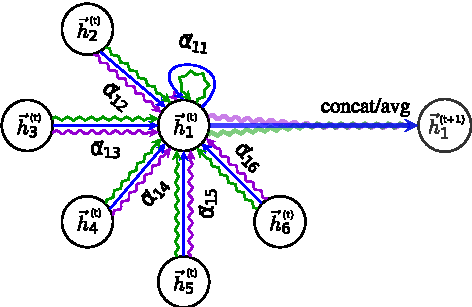
\includegraphics[width=0.5\linewidth]{images/graph_attention_network_pdfa.pdf}\\
	Figure 3.1: Illustration of multi-head attention with three heads. Different arrow colors denote independent attention mechanisms. Reproduced from \cite{veličković2018graph}
\end{center}
\par
One straightforward strategy to extend GAT on heterogeneous graphs is constructing separate learnable linear transformation $\boldsymbol{W}_{b_i}$ for each node type $b_i$ in equations \ref{equation:2.6}, \ref{equation:2.7}, \ref{equation:2.9}, projecting each node type to a shared latent space with the same dimension.

\section{Deep reinforcement learning}

For a given MDP tuple $(\mathcal{S}, \mathcal{A}, \mathcal{R}, \mathcal{P}, \gamma)$ as described in \ref{MDP for JSSP}, at each time step $t$, the agent receives a state $s_t \in \mathcal{S}$, selects an action $a_t \in \mathcal{A}$ following a policy $\pi(a_t|s_t)$, receives a reward $r_t$ and a new state $s_{t+1}$ according to the probability distribution $\mathcal{P}(s_{t+1} | s_t, a_t)$, and the cycle repeats \cite{DBLP:journals/corr/Li17b}. A sequence of states, actions, and rewards is called a trajectory. The discounted cumulative reward of the trajectory with length $T$ starting at time $t$ is the sum $G_t = \sum_{k=0}^T \gamma^k r_{t+k}$. The probability of the trajectory is $P_t = \Pi_{k=0}^T \mathcal{P}(s_{t+k+1} | s_{t+k}, a_{t+k})$. The goal of an agent is to maximize the expected discounted cumulative reward $\mathbb{E}[G_t]$ over all possible trajectories \cite{DBLP:journals/corr/Li17b}. Long term value of a state $s$ defined as $v(s) = \mathbb{E}\left [ G_t | s_t = s \right ]$ is the expected cumulative reward from the state $s$ following policy $\pi$. An optimal state value $v_*(s) = \max_\pi v_\pi(s)$ is the maximum achievable value for the state $s$. For the optimal state value, the Bellman equation holds \cite{DBLP:journals/corr/Li17b}
\begin{equation}
	v_*(s) = \max_a \sum_{s'} \mathcal{P} (s' | s,a)\left [ \mathcal{R}(s, a) + \gamma v_*(s') \right ] \, .
\end{equation}
The action-value function $q_\pi(s,a) = \mathbb{E} \left [ G_t | s_t=s, a_t=a\right ]$ is the expected cumulative reward after taking an action $a$ in state $s$ following policy $\pi$. The optimal action-value function $q_* (s,a) = \max_\pi q_\pi(s, a)$ is the maximum state-action value possible for given state $s$ and action $a$. Policy maximizing $q_\pi(s,a)$ and $v_\pi(s)$ is called optimal policy and is denoted as $\pi_*$ \cite{DBLP:journals/corr/Li17b}.
\par
Traditional algorithms for finding optimal policies include value iteration \cite{barto1989learning}, policy iteration \cite{Howard1960DynamicPA}, temporal difference learning \cite{tesauro1995temporal}, Q-learning \cite{watkins1992q}, and SARSA \cite{sarsa}.
\par
Deep reinforcement learning (DRL) methods use deep neural networks with parameters $\theta$ to approximate reinforcement learning components, such as value function $\hat{v}_\theta(s)$, action-value function $\hat{q}_\theta(s, a)$, policy $\pi_\theta(a|s)$, and also possibly state transition function and reward function \cite{DBLP:journals/corr/Li17b}. 

\subsection{Policy optimization} \label{policy_optimization}

The policy $\pi_\theta$ can be improved by performing gradient ascent w.r.t. some loss function $L(\theta)$ \cite{openai_policy_optimization}
\begin{equation}
	\theta_{k+1} = \theta_k + \alpha \nabla_\theta L(\theta)|_{\theta_k} \,
\end{equation}
where $\alpha$ is called a learning rate, and $\nabla_\theta L(\theta)$ is called the \textbf{policy gradient}. 
\par
The goal of an agent following parameterized policy $\pi_\theta$ is to maximize expected return $\mathbb{E} \left [ G_t \right ]$. Plugging in $L(\theta) = \mathbb{E} \left [ G_t \right ]$ yields \cite{openai_policy_optimization,DBLP:journals/corr/SchulmanWDRK17}
\begin{equation} \label{equation:2.12}
	\nabla_\theta L(\theta) = \mathbb{E} \left [ \sum_i \nabla_\theta \log \pi_\theta(a_i|s_i) G_t \right ] \, ,
\end{equation}
where expectation averages over a finite batch of trajectories. The cumulative reward function $G_t$ is often replaced by the advantage function $A_t$, which describes how better the action is w.r.t. other actions of the current policy, i.e., $A_t(s_t,a_t) = q_\pi(s_t, a_t) - v_\pi(s_t)$ \cite{openai_policy_optimization}. Gradient \ref{equation:2.12} is obtained from the loss function \cite{DBLP:journals/corr/SchulmanWDRK17}
\begin{equation}
	L(\theta) = \mathbb{E} \left [ \sum_i \log \theta(a_i|s_i) A_t \right ] \, .
\end{equation}
Authors of \textbf{Proximal Policy Optimization} (PPO) algorithm \cite{DBLP:journals/corr/SchulmanWDRK17} propose the following loss function
\begin{equation}
	L(\theta) = \mathbb{E}_t \left [ \min \left( r_t(\theta) \hat{A_t} , \text{clip}(r_t(\theta), 1-\epsilon, 1+\epsilon) \hat{A_t} \right) \right ] \,
\end{equation}
where $r_t(\theta) = \frac{\pi_\theta(a_t|s_t)}{\pi_{\theta_\text{old}}(a_t|s_t)}$ is the probability ratio with $r(\theta_\text{old}) = 1$, and $\epsilon$ is a hyperparameter, which authors set to $\epsilon = 0.2$ \cite{DBLP:journals/corr/SchulmanWDRK17}. $\hat{A_t}$ is an advantage estimate \cite{DBLP:journals/corr/SchulmanWDRK17}
\begin{equation}
	\hat{A_t} = \delta_t + (\gamma \lambda) \delta_{t+1} + \cdots + (\gamma\lambda)^{T - t + 1} \delta_{T - 1} \, ,
\end{equation}
where $\delta_t = r_t + \gamma v(s_{t+1}) - v(s_t)$, $\lambda$ is a hyperparameter, and $t \in \left [ 0, T \right ]$.
\par
The full PPO algorithm is shown below \cite{DBLP:journals/corr/SchulmanWDRK17}. In each iteration, $N$ actors collect $T$ timesteps of data. Then, the surrogate loss of these $NT$ timesteps of data is calculated and parameters $\theta$ are optimized.

\begin{algorithm}[H]
	\caption{Proximal Policy Optimization algorithm}\label{algorithm:ppo}
	\begin{algorithmic}[1]
	\renewcommand{\algorithmicrequire}{\hspace*{\algorithmicindent}  \textbf{Input:}}
	\renewcommand{\algorithmicensure}{\hspace*{\algorithmicindent}  \textbf{Output:}}
	\Require Environment
	\Ensure Trained policy 
	\State $\pi_{\theta_\text{old}} \gets$ initialize random policy
	\For{iteration$=1,2,...$ }
		\For{actors$=1,2,...,N$}
			\State Run Policy $\pi_{\theta_\text{old}}$ in environment for $T$ timesteps
			\State Compute advantage estimates $\hat{A_1}$, ..., $\hat{A_T}$
		\EndFor
		\State Optimize $L$ wrt $\theta$, with $K$ epochs and minibatch size $M \leq NT$
		\State $\theta_{\text{old}} \gets \theta$
	\EndFor
	\State return $\pi_{\theta_\text{old}}$
\end{algorithmic}
\end{algorithm}

\subsection{Deep Q-network} \label{dqn}

Deep Q-network (DQN) is an algorithm using a neural network to approximate the action-value function $\hat{q}_\theta(s, a)$ \cite{mnih2015human}. It also stores agent's experience as tuples $e_t = (s_t, a_t, r_t, s_{t+1})$ in a data set $D_t = \{e_1, ..., e_t\}$. During training, Q-learning updates are performed on samples drawn uniformly from the agent's experience $D$ to reduce correlation in the trajectories observations \cite{mnih2015human}. The Q-learning update uses the following loss function \cite{mnih2015human}
\begin{equation} \label{equation:2.16}
	L_i(\theta_i) = \mathbb{E} \left [\left ( r + \gamma \max_{a'}\hat{q}_{\theta^-_i}(s',a') -\hat{q}_{\theta_i}(s,a) \right )^2 \right ] \, ,
\end{equation}
where the expectation is with respect to the batch of $e_t$,
$\hat{q}_{\theta_i}(s,a)$ is the Q-network at iteration $i$, and $\hat{q}_{\theta^-_i}(s,a)$ is the target network used to compute targets at iteration $i$. The target network is updated with the Q-network parameters every $C$ step and fixed between updates. The full algorithm is shown below \cite{mnih2015human}.

\begin{algorithm}[H]
	\caption{Deep Q-learning with experience replay} \label{algorithm:dqn}
	\begin{algorithmic}[1]
	\renewcommand{\algorithmicrequire}{\hspace*{\algorithmicindent}  \textbf{Input:}}
	\renewcommand{\algorithmicensure}{\hspace*{\algorithmicindent}  \textbf{Output:}}
	\Require Emulator
	\Ensure Action-value function
	\State Initialize replay memory $D$ to capacity $N$
	\State Initialize action-value function $\hat{q}_\theta$ with random weights
	\State Initialize target action-value function $\hat{q}_{\theta^-} = \hat{q}_\theta$
	\For{episode $=1,...,M$}
		\State Initialize sequence $s_1 = \{x_1\}$ and preprocessed sequence $\phi_1 = \phi(s_1)$
		\For{t $=1,...,T$}
			\State With probability $\varepsilon$ select a random action $a_t$
			\State otherwise select $a_t = \text{argmax}_a \hat{q}_\theta(\phi(s_t), a)$
			\State Execute action $a_t$ in emulator and observe reward $r_t$ and image $x_{t+1}$
			\State Set $s_{t+1} = s_t, a_t, x_{t+1}$ and preprocess $\phi_{t+1} = \phi(s_{t+1})$
			\State Store transition $(\phi_t, a_t, r_t, \phi_{t+1})$ in $D$
			\State Sample random minibatch of transitions $(\phi_j, a_j, r_j, \phi_{j+1})$ from $D$
			\State Set $ y_j = \begin{cases} r_j & \mbox{if episode ends at step } j+1 \\ r_j + \gamma \max_{a'}\hat{q}_{\theta^-}(\phi_{j+1}, a') & \mbox{otherwise} \end{cases}$
			\State Perform a gradient descent step on $(y_j - \hat{q}_\theta(\phi_j, a_j))^2$ w.r.t to $\hat{q}_\theta$
			\State Every $C$ steps reset $\hat{q}_{\theta^-} = \hat{q}_{\theta}$
		\EndFor
	\EndFor
	\State return $\hat{q}_\theta$
\end{algorithmic}
\end{algorithm}

The max operator in equation \ref{equation:2.16}, also present in standard Q-learning algorithm \cite{watkins1992q}, uses the same action-value function to select and evaluate the action, leading to overoptimistic value estimates. To counteract this, in Double Q-learning \cite{hasselt2010double}, two value functions are learned by randomly choosing which to update. During each update, one function selects a greedy action, and the other determines its value. Using this mechanism in DQN algorithm \ref{algorithm:dqn} leads to an algorithm called \textbf{Double DQN} \label{Double DQN} \cite{Hasselt_Guez_Silver_2016} (DDQN), as a reference to both Double Q-learning and DQN. DDQN replaces expression for target $y_j$ in case \textit{"otherwise"} on line 13 in algorithm \ref{algorithm:dqn} with \cite{Hasselt_Guez_Silver_2016}
\begin{equation}
	y_j = r_j + \gamma \hat{q}_{\theta^-}(\phi_{j+1}, \text{argmax}_a \hat{q}_\theta(\phi_{j+1}, a)) \, .
\end{equation}
The Q-network selects the action, and the target network estimates its value.
